\documentclass{article}
\usepackage[utf8]{inputenc}
\usepackage{amsmath}
\usepackage{amssymb}
\usepackage{amsthm}
\usepackage{cancel}
\usepackage[shortlabels]{enumitem}
\usepackage{caption}
\usepackage{graphicx}
\usepackage[top=0.5in, bottom=0.5in, left=1in, right=1in]{geometry}
\usepackage{float}

% \usepackage{titlesec}
%     \titlespacing{\subsection}{\parindent}{15pt}{12pt}

\title{\textbf{\underline{CSCI4150U: Data Mining}\\Lab 04}}
\author{Syed Naqvi\\100590852}
\date{\today}

\begin{document}

    \maketitle
    
    \section*{Part I:}

    \subsection*{1. Preprocessing (German Credit Data)}
    
    This dataset contains a mixture of ordinal, nominal and numeric features. The ordinal and nominal
    features must be processed such that Minkowski distance provides a meaningful metric
    during k nearest neighbors classifications while retaining as much information as possible.
    We begin with the following features which have either a completely arbitrary ordering or
    contain only 2 unique values:

    \begin{itemize}
        \item attribute 4: Purpose
        \begin{itemize}
            \item a list of purchases on credit
        \end{itemize}
        \item attribute 9: Personal status and sex
        \begin{itemize}
            \item an arbitrarily ordered list of marital status and sex
        \end{itemize}
        \item attribute 19: Telephone
        \begin{itemize}
            \item either have a Telephone (yes) or do not (no)
        \end{itemize}
        \item attribute 20: Foreign worker
        \begin{itemize}
            \item either is a foreign worker (yes) or is not (no)
        \end{itemize}
    \end{itemize}
    
    \newpage

    We can use \textbf{one-hot encoding} for Attributes 4 and 9 as these features have multiple
    unique values and \textbf{label encoding} for attributes 19 and 20 as these features have
    only two unique values which makes ordering of label encoding irrelevant.

    \begin{figure}[H]
        \centering
        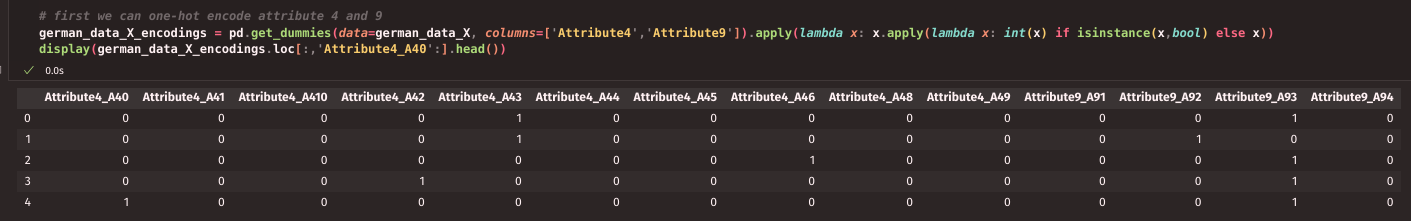
\includegraphics[width=\textwidth, height=0.13\textheight]{./I_1_g_a.png}
        \caption{[Attributes 4 and 9 one-hot encoding]}
    \end{figure}
    \begin{figure}[H]
        \centering
        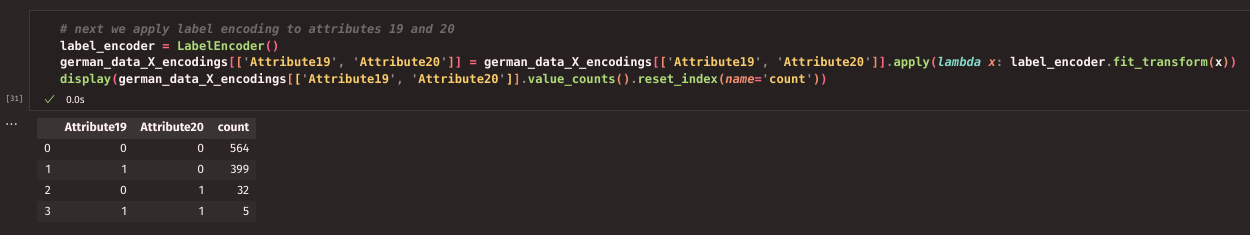
\includegraphics[width=\textwidth, height=0.13\textheight]{./I_1_g_b.png}
        \caption{[Attributes 19 and 20 label encoding]}
    \end{figure}

    The next set of features appear to have a clear ordinal ranking with least credit-worthy
    on the left to most credit-worthy on the right:
    \begin{itemize}
        \item Attribute 1: Status of existing checking account
        \begin{itemize}
            \item A11 ($<$ 0 DM) $\to$ A12 (0 $<=$ \& $<$ 200 DM) $\to$ A13 ($>=$ 200 DM / salary assignments for at least 1 year) $\to$ A14 (no checking account)
        \end{itemize}
        \item Attribute 3: Credit history
        \begin{itemize}
            \item A34 (critical account / other credits existing) $\to$ A33 (delay in paying off in the past) $\to$ A32 (existing credits paid back duly till now) $\to$ A31 (all credits at this bank paid back duly) $\to$ A30 (no credits taken / all credits paid back duly)
        \end{itemize}
        \item Attribute 6: Savings account / bonds
        \begin{itemize}
            \item A61 ($<$ 100 DM) $\to$ A62 (100 $<=$ \& $<$ 500 DM) $\to$ A63 (500 $<=$ \& $<$ 1000 DM) $\to$ A64 ($>=$ 1000 DM) $\to$ A65 (unknown / no savings account)
        \end{itemize}
        \item Attribute 7: Present employment since
        \begin{itemize}
            \item A71 (unemployed) $\to$ A72 ($<$ 1 year) $\to$ A73 (1 $<=$ \& $<$ 4 years) $\to$ A74 (4 $<=$ \& $<$ 7 years) $\to$ A75 ($>=$ 7 years)
        \end{itemize}
        \item Attribute 12: Property
        \begin{itemize}
            \item A124 (unknown / no property) $\to$ A123 (car or other, not in attribute 6) $\to$ A122 (building society savings agreement / life insurance) $\to$ A121 (real estate)
        \end{itemize}
        \item Attribute 17: Job
        \begin{itemize}
            \item A171 (unemployed / unskilled - non-resident) $\to$ A172 (unskilled - resident) $\to$ A173 (skilled employee / official) $\to$ A174 (management / self-employed / highly qualified employee / officer)
        \end{itemize}
    \end{itemize}

    \newpage
    
    We can visualize the value distributions of each feature for each class:
    

    % \begin{figure}[H]
    %     \centering
    %     \begin{minipage}[t]{0.47\textwidth}
    %         \centering
    %         % \includegraphics[width=\textwidth, height=0.35\textheight]{}
    %         \caption{Decision tree performance based on holdout method and Gini impurity using Statlog German Credit Dataset}
    %     \end{minipage}
    %     \hfill
    %     \begin{minipage}[t]{0.47\textwidth}
    %         \centering
    %         % \includegraphics[width=\textwidth, height=0.35\textheight]{}
    %         \caption{Decision tree performance basd on holdout method and Gini impurity using Waveform Dataset}
    %     \end{minipage}
    % \end{figure}

    \newpage

\end{document}